\section{Eingesetzte Tools}
Im folgenden Abschnitt soll ein kurzer Überblick über die verschiedenen eingesetzten Tools gegeben werden. Diese Beschreibung ist nicht vollständig da Grundkentnisse (wie kompilieren eines Linux Kernels aus den Sourcen) vorausgesetzt werden.

\subsection{\ac{FPGA} Entwicklung}

\subsubsection{Quartus}
Das Tool Quartus bildet die Grundlage um für Altera (bzw. inzwischen Intel) \acp{FPGA} entwickeln zu können. Im Prinzip ist es eine Sammlung von verschiedenen Tools, die über eine GUI gesteuert werden. Alle relevanten Prozesse (Building, Generieren von IP-Cores, Systemanalyze etc.) sind auch (u.U. sogar mächtiger) als Kommandozeilentools verfügbar. Das vollständige Handbuch ist unter \href{https://www.altera.com/en_US/pdfs/literature/hb/qts/qts-qps-handbook.pdf}{Quartus Handbuch} zu finden (Achtung: 1939 Seiten!, und das ist nur der erste Teil). Als Überblick und um mit dem Garfield Projekt zu starten gibt es einige nützliche Links und Tutorials wie z.B. \href{https://www.altera.com/support/training/university/materials-tutorials.html}{Altera University Programm - Start}. Eine weitere, sehr empfehlenswerte Anlaufstelle bei Problemen oder auf der Suche nach Application Notes, Tutorials, HowTos und auch Vorträgen ist \href{rocketboards.org}{rocketboards.org}. Dabei handelt es sich um die offizielle Open-Source Sammlung rund um Intel \acp{FPGA}.\\

Die OTH hat eine Reihe von Lizenzen für die gesamte Altera Toolchain (Quartus, SoC EDS, IP-Cores etc.). Wird das Garfield Projekt mit der unlenzierten Version syntethisiert, kompiliert Quartus automatisch einen \textquotedblleft Ablaufzeitstempel\textquotedblright~mit ins Design. Der NIOS2 Prozessor und einige \ac{IP}-Cores sind damit nur ca. 30 Minuten lauffähig! Die Lizenzen verwaltet Herr Altmann. Dieser hat auch mind. einen WLAN-USB Stick an dessen MAC-Addresse die Lizenz gebunden ist. Es ist nicht empfehlenswert die Lizenz an eine feste MAC-Addresse eines privaten PCs zu binden, da diese Lizenz dann für andere Studenten verbraucht wäre. Die Installation von Quartus sollte im Hochschulnetz erfolgen da die Downloadgröße ca. 20GB beträgt.

\subsubsection{Qsys}
Bei QSYS handelt es sich um Intels System Integrations Tool. Es ist eine sehr abstrakte Variante sich ein komplettes \ac{FPGA} System zusammenzuklicken und automatisch jegliche Hardwarebeschreibungen, evtl. notwendige Treiber für den NIOS2 etc. zu generieren. Nach der Generierung entsteht ein großer IP-Core, der abschließend in die eigene Pinbeschreibung eingebettett werden muss. Auch für dieses Tool kann am besten wieder auf ein Tutorial \href{https://www.altera.com/content/dam/altera-www/global/en_US/pdfs/literature/tt/tt_qsys_intro.pdf}{QSYS Tutorial} oder auf \href{rocketboards.org}{rocketboards.org} hingewiesen werden.
Da das Garfield Projekt auch zwei selbstgeschriebenen Hardwarekomponenten beinhaltet, müssen die Pfade für diese QSYS bekanntgemacht werden. Dies ist nicht nur notwendig für die Person, die das Hardwaredesign anpasst/syntethisiert, sondern auch für Beteiligte, die Code für den NIOS2 schreiben wollen und auf die \ac{HAL}-Generierung des Tools angewiesen sind. Dazu müssen in QSYS die Einstellungen wie in Abbildung \ref{Settings:IP} dargestellt. Bei geöffnetem QSYS muss unter \texttt{Tools->Options->IP Search Path}.

\begin{figure}
	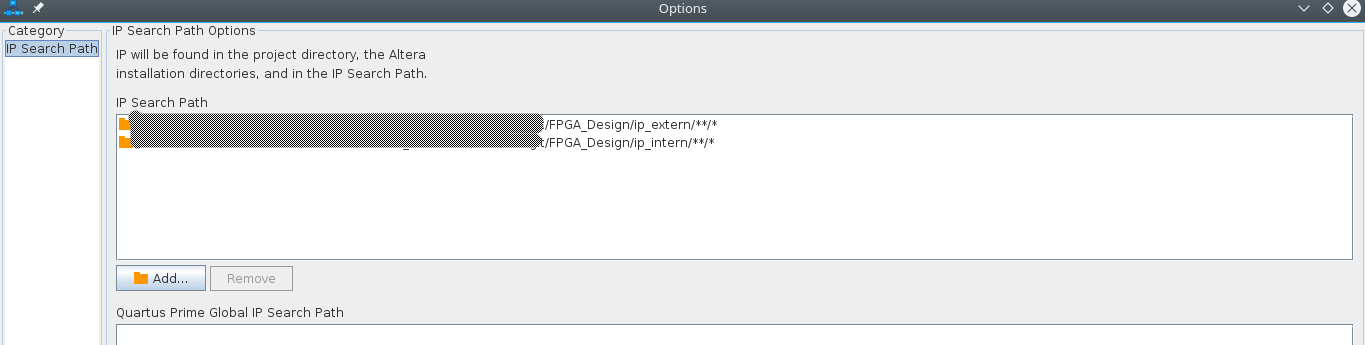
\includegraphics[width=\textwidth]{Abb/Qsys_settings.png}
	\caption{Einstellungen für die selbstgeschriebenen \ac{IP}-Cores}
	\label{Settings:IP}
\end{figure}

\subsubsection{Quartus Programmer}
Der Quartus Programmer dient dazu, entweder das \ac{FPGA} direkt mit der entsprechenden Image Datei (\texttt{*.sof}-Endung) oder das angeschlossene Flash mit einer \texttt{*.jic} Datei zu flashen. In den entsprechenden Quartus Tutorials sind auch kleine HowTos enthalten, wie mit dem Programmer umzugehen ist. Auf der für das Board zugeschnittene \href{http://www.terasic.com/downloads/cd-rom/de0-nano-soc/}{System-CD} befindet sich auch eine \texttt{DE0-Nano-SoC\_User\_manual.pdf}. In diesem ist auch beschrieben, wie man eine Datei für den Flash erstellt und dies auf den Flash lädt.